\documentclass[14pt, a4paper]{article}  % Любой документ начинается с такой строки! В ней мы выбираем 
\author{Голованова Лиза}
\usepackage{amsmath,amsfonts,amssymb,amsthm,mathtools}  % Тут мы подключаем пакеты для математики!
\usepackage{graphicx}
\graphicspath{{Pics/}}
\DeclareGraphicsExtensions{.pdf,.png,.jpg}
\usepackage{fontspec}         % пакет для подгрузки шрифтов
\setmainfont{Roboto}          % задаёт основной шрифт документа

\usepackage{unicode-math}     % пакет для установки математического шрифта
\setmathfont{Asana Math}      % шрифт для математики

\usepackage{polyglossia}      % Пакет, который позволяет подгружать русские буквы
\setdefaultlanguage{russian}  % Основной язык документа
\setotherlanguage{english}    % Второстепенный язык документа
\usepackage{tipa}
\usepackage{mathrsfs}
\usepackage{subfigure}
\usepackage{rotating}
\usepackage{tikz}

\begin{document}
\begin{figure}[!htb]
\minipage{0.32\textwidth}
  
\includegraphics[width=0.8\linewidth]{pop3.pdf}
\endminipage\hfill
\minipage{0.32\textwidth}
  \includegraphics[width=0.8\linewidth]{pop5.pdf}
\endminipage\hfill
\minipage{0.32\textwidth}%
  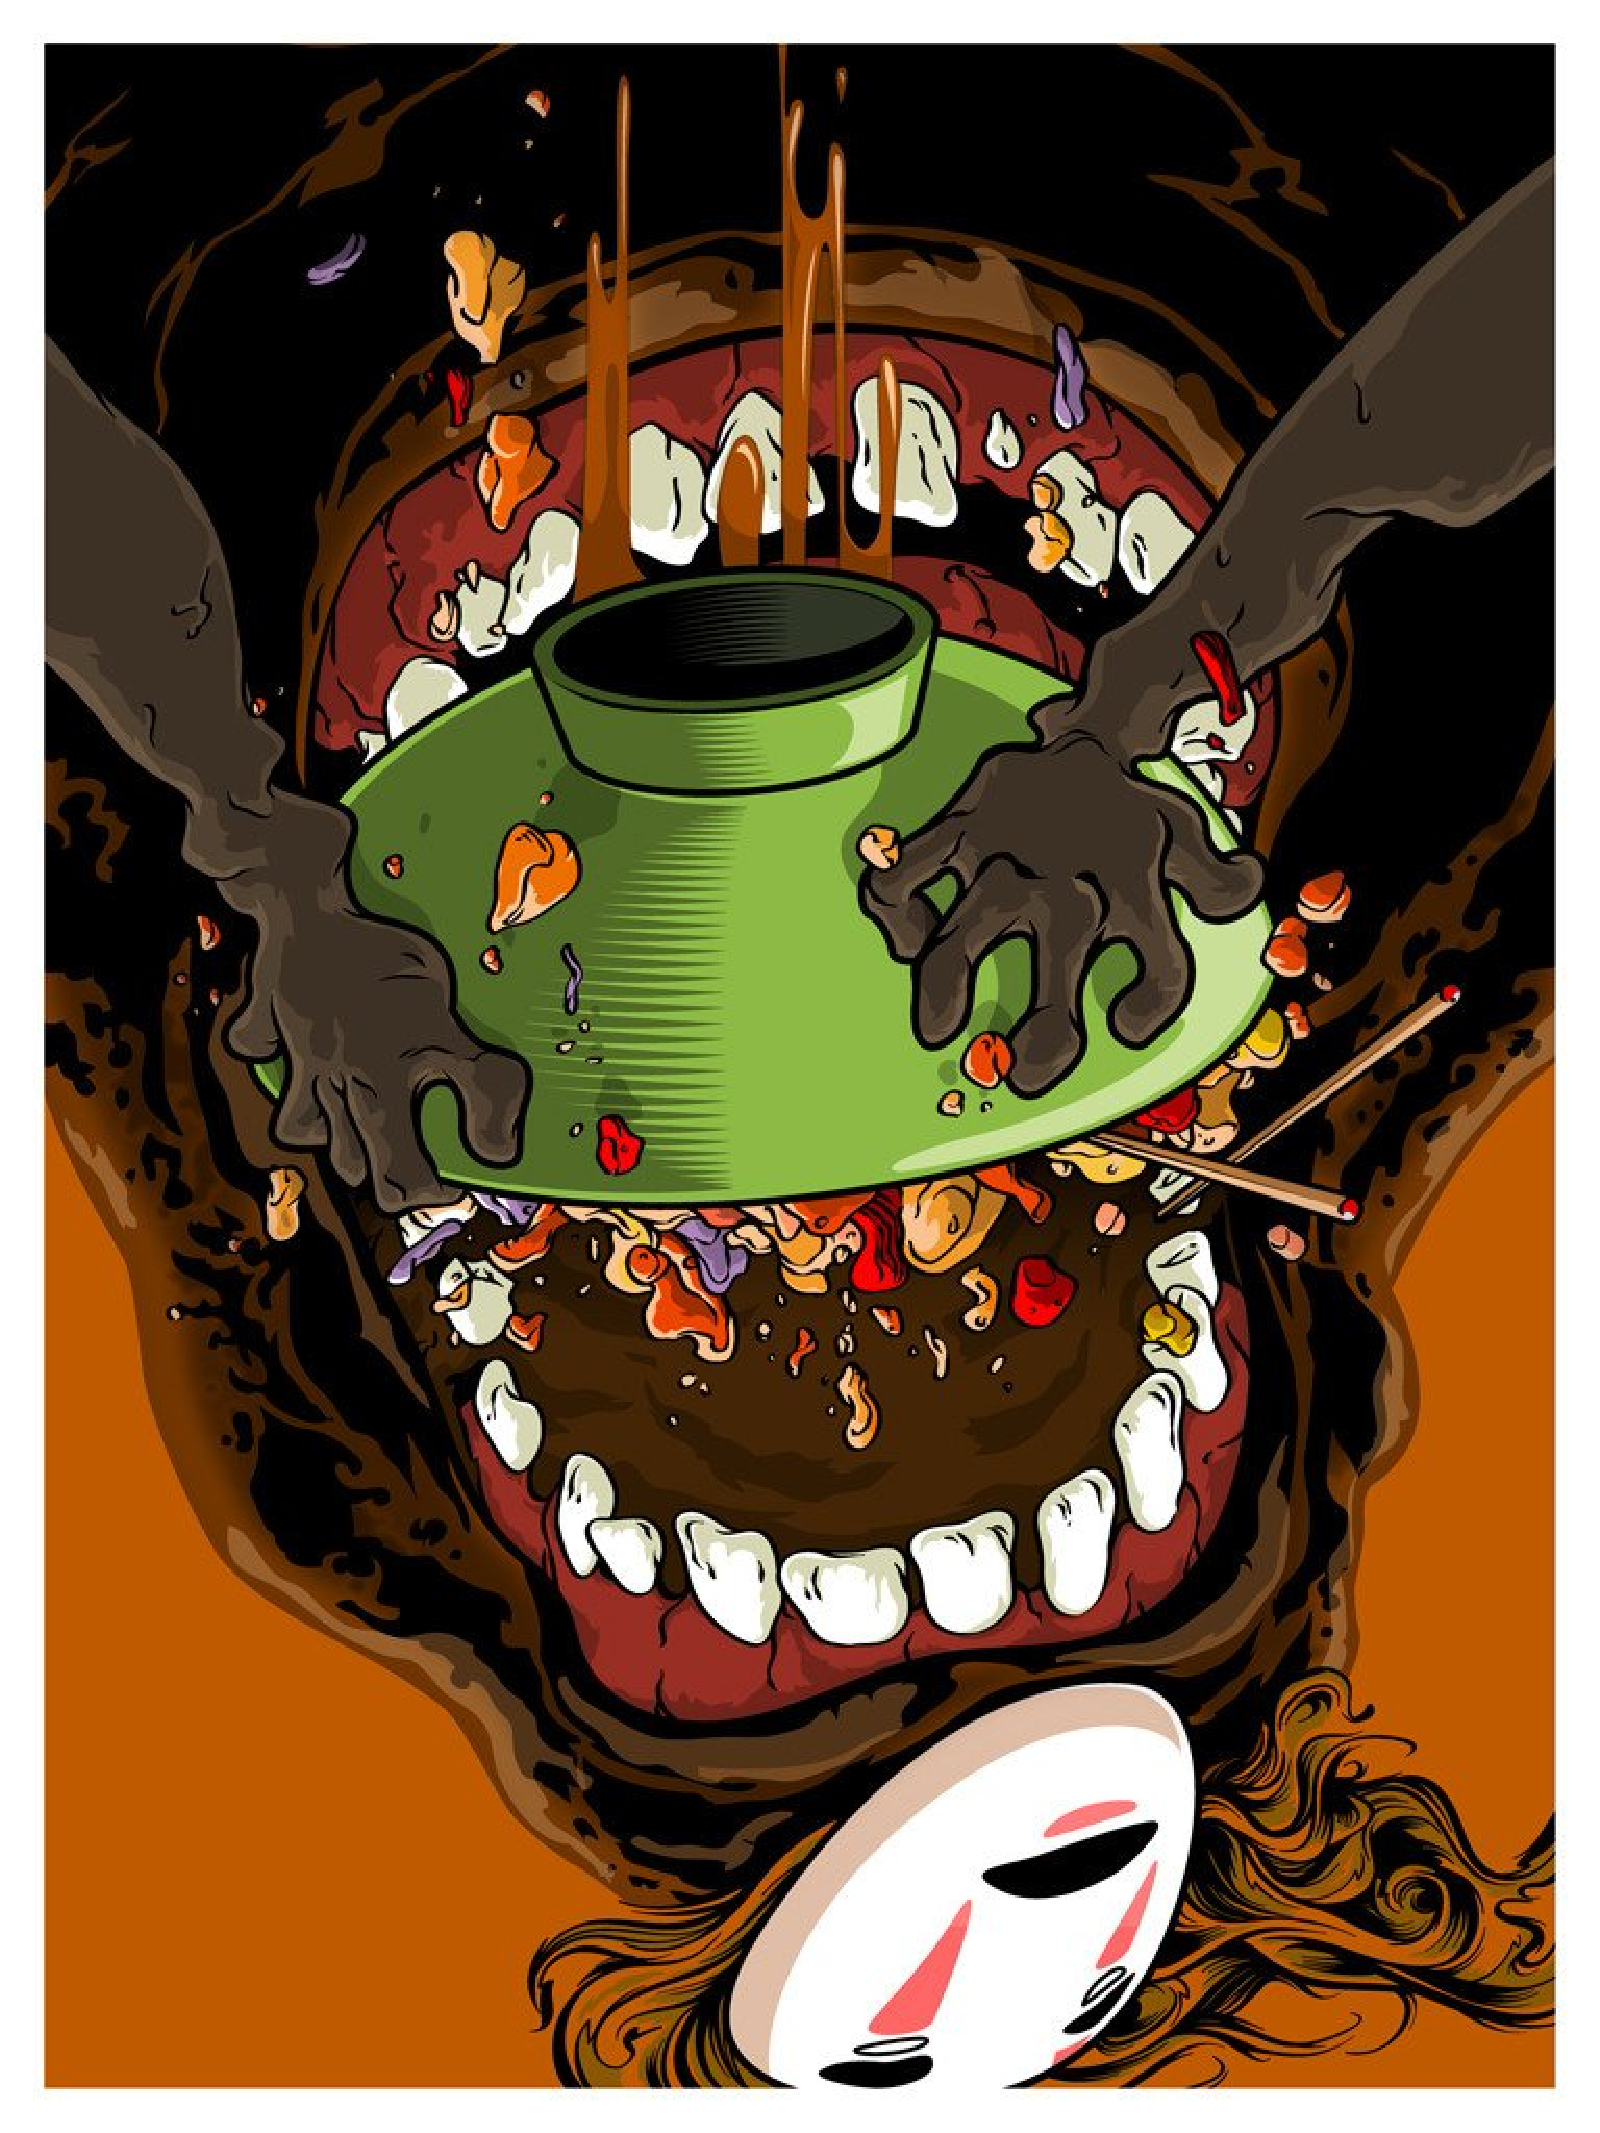
\includegraphics[width=0.8\linewidth, angle=180]{pop6.pdf}
\endminipage\vfill
\minipage{0.32\textwidth}
  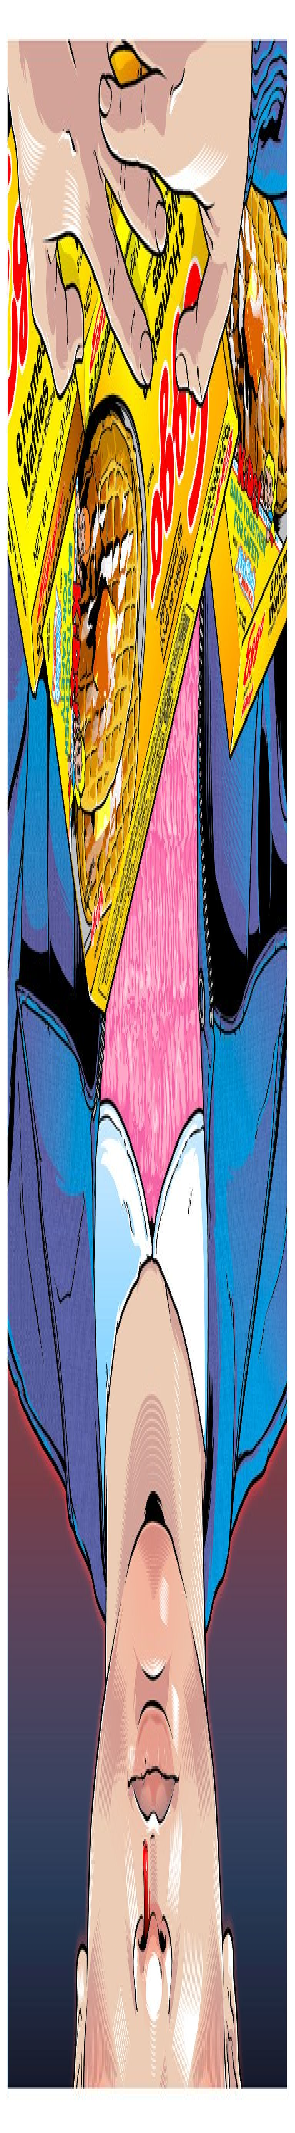
\includegraphics[width=0.8\linewidth, height=1.075\linewidth, angle=180]{pop2.pdf}
\endminipage\hfill
\minipage{0.32\textwidth}\hspace*{-2.1cm}
  
\includegraphics[width=0.24\linewidth, angle=45, height=1.85\linewidth, keepaspectratio]{pop4.pdf}
\endminipage\hfill
\minipage{0.32\textwidth}\hspace*{-1.85cm}
  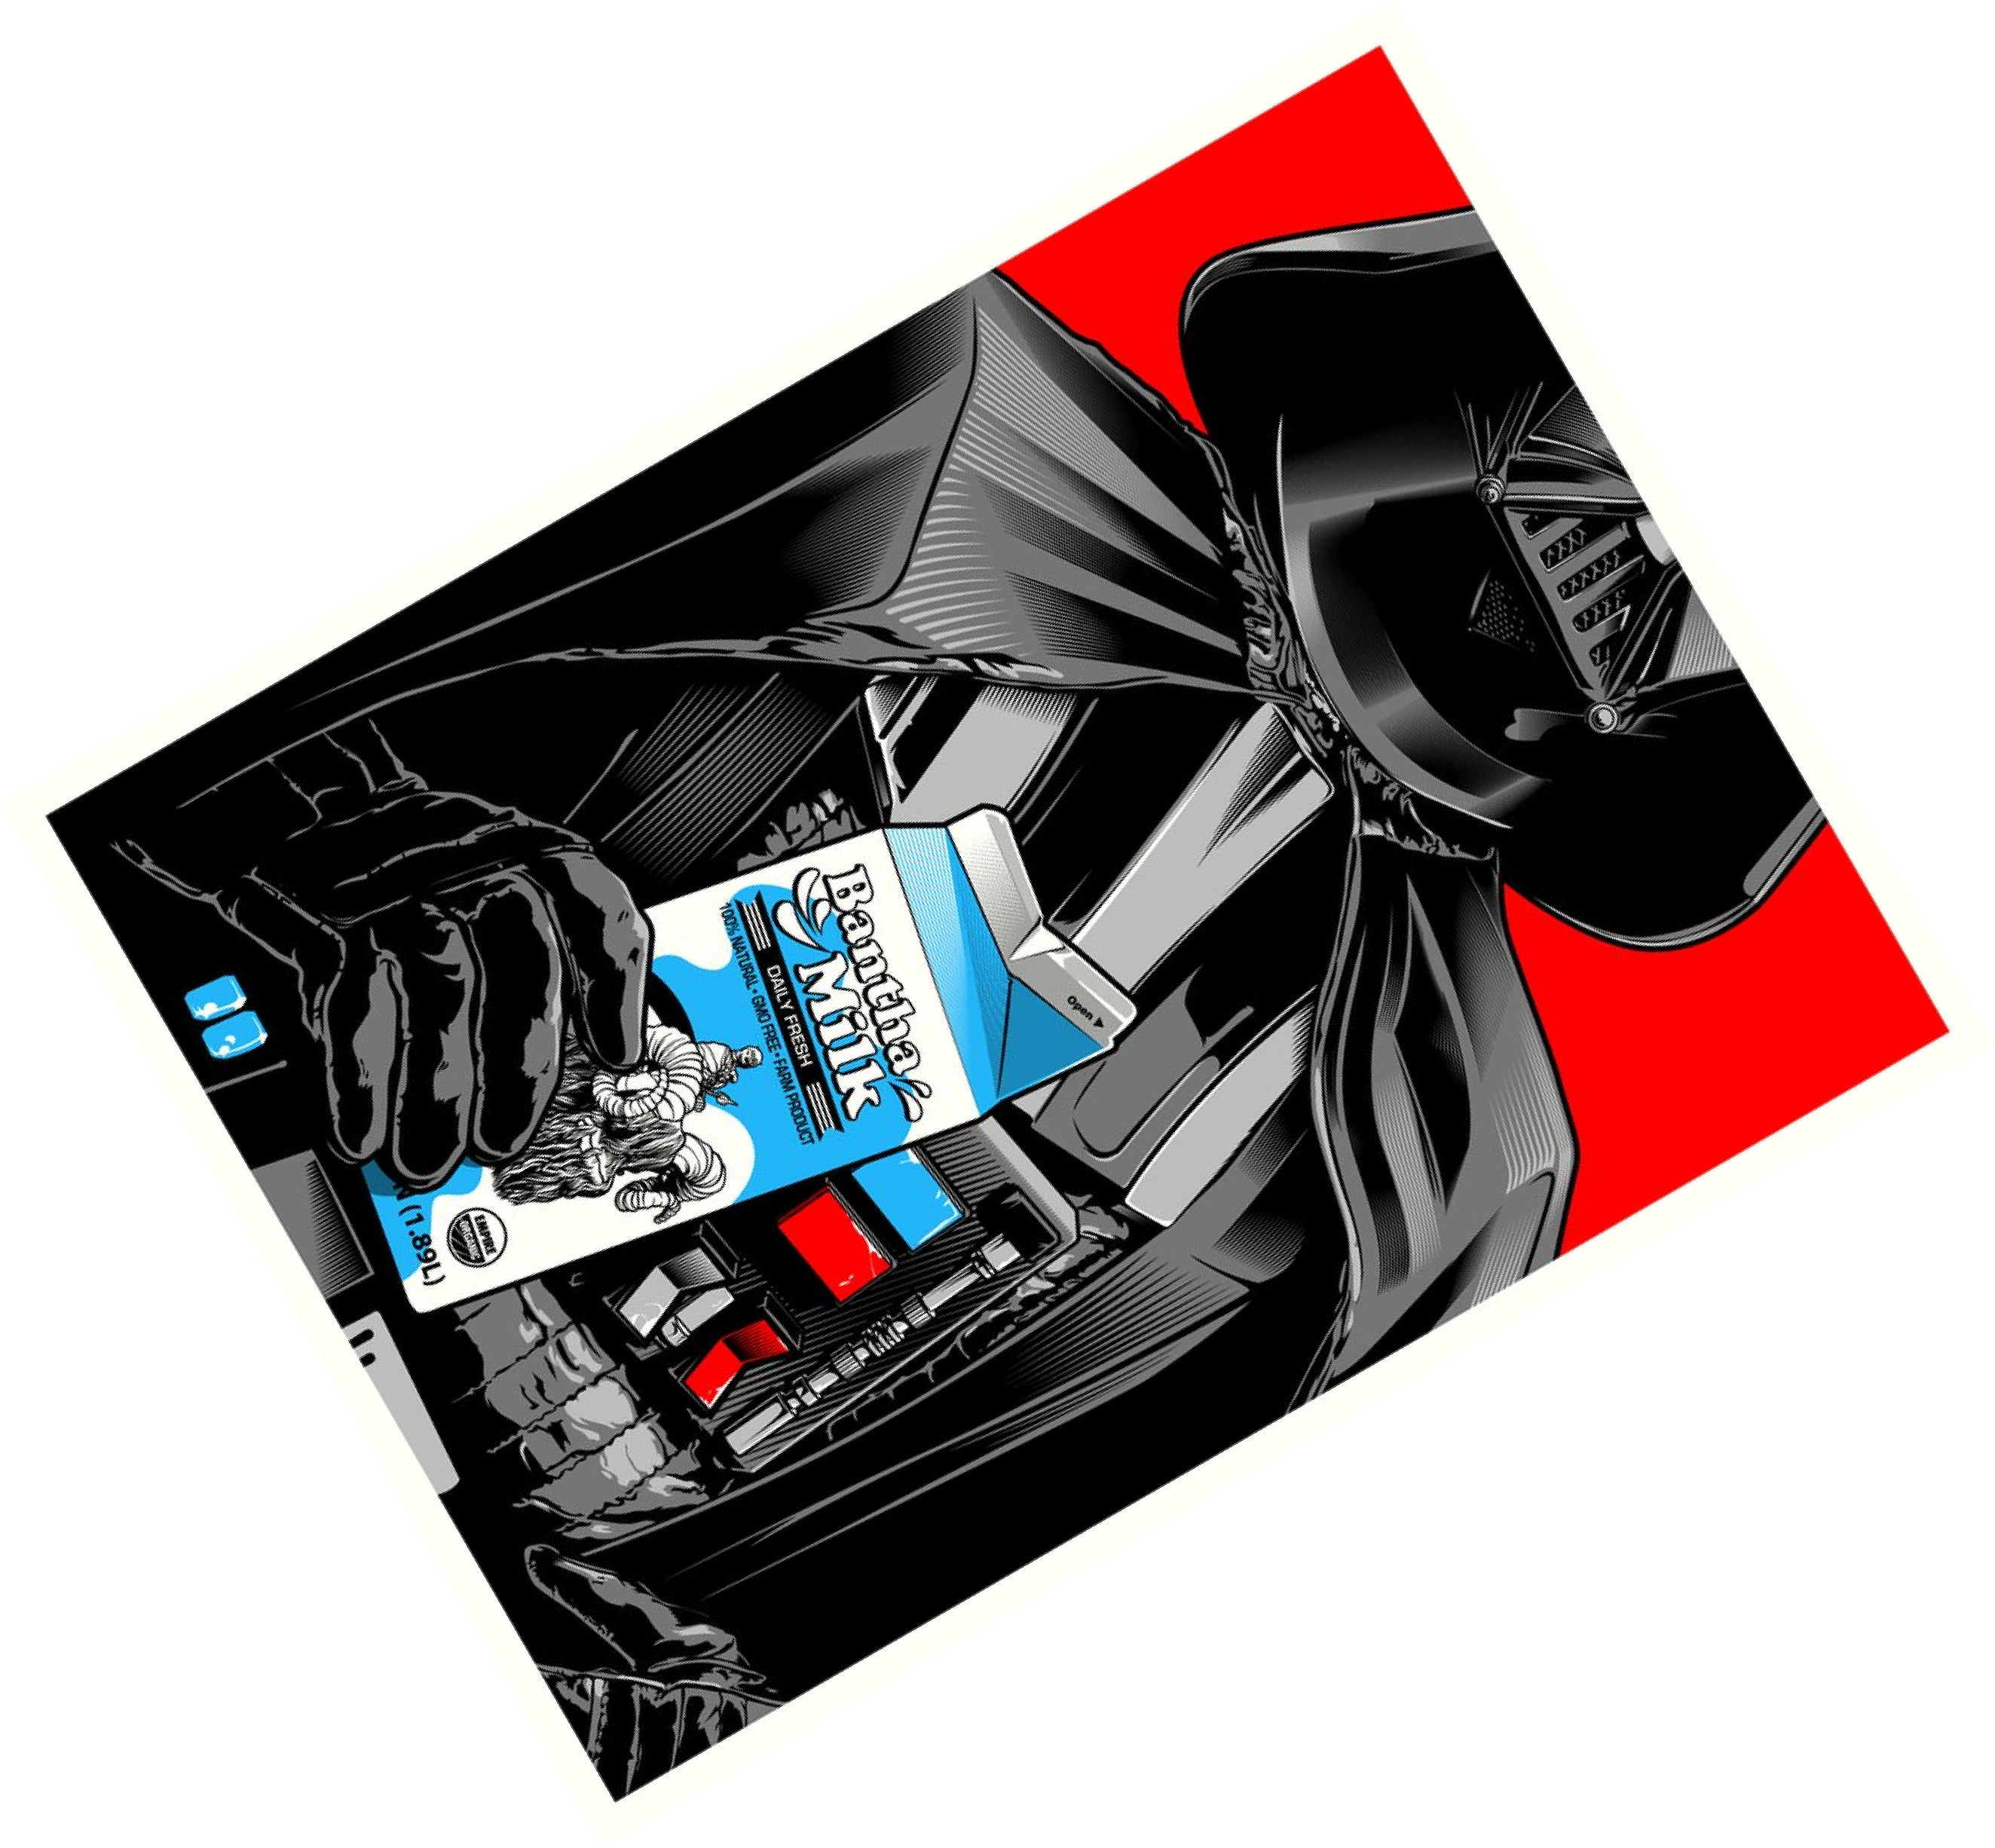
\includegraphics[width=0.24\linewidth, angle=60,  height=1.75\linewidth, keepaspectratio]{pop9.pdf}
\endminipage
\caption{Поп-арт к вашим услугам}
\end{figure}

\end{document}